\chapter{Estratégias de Abordagem aos Problemas} \label{cap:abordagem}
Nesta secção vamos analisar os procedimentos, tecnologias e conceitos utilizados no desenvolvimento deste projeto.

\section{Modelo de Dados} \label{sec:dados}
Um dos componentes deste sistema é um repositório de dados, que irá conter as várias informações relacionadas com os clientes deste serviço. Na figura \ref{fig:relacoes} estão representados os vários elementos deste modelo de dados. \\

\begin{figure}[ht!]
\centering
\resizebox{105mm}{!}{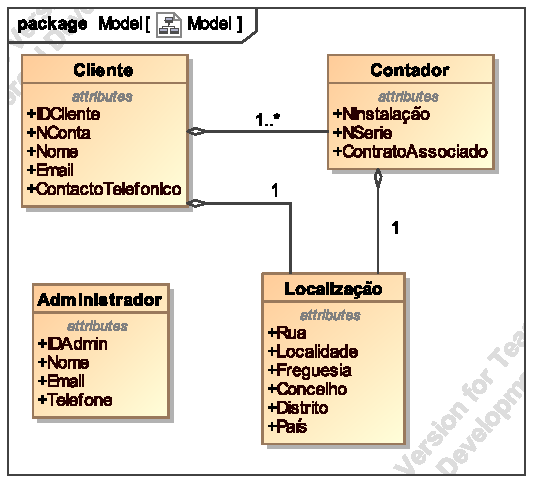
\includegraphics{diagramas/svg/uml__Model.pdf}}
\caption{Arquitetura do sistema.}
\label{fig:relacoes}
\end{figure}

O elemento utilizador representa um utilizador do sistema. Para cada utilizador será registado um ID único, o seu nome, email e número de telefone/telemóvel. Os utilizadores podem ser utilizadores administradores ou podem ser clientes. Os clientes, para além dos dados registados como utilizador, têm também o seu número de cliente e número de conta e a sua morada. \\
Os utilizadores terão associado um ou mais contadores, pelo que para cada contador guardamos o seu número único de instalação, o seu número de série e o contrato ao qual ele está associado. \\
Cada contador tem uma localização, que representa o local onde o contador está instalado. Cada cliente tem também uma localização associada, que representa a sua morada principal para onde é, por exemplo, enviado o correio postal. Uma localização segue a estrutura normal de uma morada: rua, localidade, freguesia, concelho, distrito e país.

